\documentclass{article}
\usepackage{xcolor}
\usepackage{listings}

\definecolor{codegreen}{rgb}{0,0.6,0}
\definecolor{codegray}{rgb}{0.5,0.5,0.5}
\definecolor{codepurple}{rgb}{0.58,0,0.82}
\definecolor{backcolour}{rgb}{0.95,0.95,0.92}

\lstdefinestyle{mystyle}{
    backgroundcolor=\color{backcolour},
    commentstyle=\color{codegreen},
    keywordstyle=\color{magenta},
    numberstyle=\tiny\color{codegray},
    stringstyle=\color{codepurple},
    basicstyle=\ttfamily\footnotesize,
    breakatwhitespace=false,
    breaklines=true,
    captionpos=b,
    keepspaces=true,
    numbers=left,
    numbersep=5pt,
    showspaces=false,
    showstringspaces=false,
    showtabs=false,
    tabsize=2
}

\lstset{style=mystyle}


\usepackage{hyperref}

\hypersetup{
    colorlinks=true,
    linkcolor=blue,
    filecolor=magenta,
    urlcolor=cyan,
    pdftitle={Document},
    pdfpagemode=FullScreen,
}

\usepackage{graphicx}
\usepackage{float}

\title{Emulation}
\author{Takanen Edoardo}
\begin{document}

\maketitle
\begin{center}
\LARGE
Abstract \

\end{center}
As a kid, I used to play with some Nintendo (copyright symbol) consoles like the Wii or the DS and I've always been keen about the games they make. This passion for videogames grew on me so that I got interested in the making process of them, leading to game development. I never asked myself one question, though, until this year, which is how are these games able to run onto this consoles? and how can people make emulators so that I could play on my personal computer? Thus, I decided to embrace the unknown world of emulation, because I have always been fascinated by it and always took it for granted.
\newpage
\tableofcontents
\newpage
\section{Introduction}\label{sec:introduction}

Emulation is not well explained on the Internet. Mainly, the results you will find if you search for it are "the program pretends to be the console" or "you will be able to play old titles". I was not satisfied with these responses, I wanted to know more. Thus, my emulation journey started with looking for a full definition of this process. I will try to give my own definition of emulation, so that I can lay a starting point to a general knowledge that will be then deepened during the paper. With this being said, to "make an emulator" means to develop the software that will do exactly what the hardware of the console does, so that when plugging the game data, the program will know how to read and handle it. \\
Emulation can only happen when the machine in which we run the software is more powerful than the hardware we want to emulate. For example, if our console has 2Kb of memory, for sure we are not able to emulate it on a computer that has 2Kb or less, since we also have to consider that the host computer will have an operating system running (which uses some of the RAM). I chose to make a Gameboy emulator, because while looking for the retro consoles, it seemed the least difficult when talking about the hardware structure complexity, meaning a good way to start tackling this subject.
\newpage
\section{Premises}\label{sec:premises}

This emulator project is purely for understanding the concepts and the theory about how a machine like a console (or similarly a computer) is made (and also for fun). There are many better-developed Gameboy emulators online, and making one that could compete with the other popular ones is nowhere near my goals. Therefore, I could not achieve the level of knowledge I want to reach if I just looked at other people's codes, I want to \textbf{fully} understand the subject. Obviously though I have to start somewhere, I do not have the skills to reverse-engineer a real Gameboy (although it would be an extremely interesting challenge), for this reason I will only consult theory guides made by many passionate developers and hackers that already did the work of studying the Gameboy from scratch for us. For a better understanding, I used two sources for this project, in order to have a dual perspective on the study.\\
For anyone who would like to dig into this challenge, the guides are
\href{https://gbdev.io/}{GBDev}  and
\href{https://hacktix.github.io/GBEDG/}{GBEDG}. \\
\\
What this paper is not. \\
This paper is not and was not intended as a guide, I previously attached some real references. This document is a report of my journey throught the development of the emulator, made for understanding the fundamentals of what is around us, from personal computers to smartphones. It could also be a way for readers to get passionate about this topic and an inspiration for them to make their own emulators (or even better, their own consoles!).
\newpage
\section{General Structure}\label{sec:general-structure}

The first thing I want to cover is in what way we want to structure our emulator.
\lstinputlisting[language=C++,label={lst:general-structure}]{./code/general-structure.code}
Actually, when we look at the circuit inside the Gameboy, all the components are, on one side, all on their own, they all execute at the same time. The CPU could be executing a simple addition, while the PPU could be rendering graphics onto the screen, all of these things happen simultaneously. This \textbf{can} be done with software, but would mean more complexity. Hence we will pick a less complicated path, and decide to execute the components one at a time.
\lstinputlisting[language=C++,label={lst:clocking}]{./code/clocking.code}
The real hardware is driven by the clock, while my implementation will be driven by how many clock cycles an instruction took.
\newpage
Before looking at the main components that shape the Gameboy hardware, I would like to focus on how memory is subdivided inside the console.\\
The address bus had 16 bits, meaning there could be 65'536 unique addresses (64Kb). \\
Since the Gameboy did not have a flash memory, those 64Kb were all the console could access (this includes all the different RAMs, the cartridge data, and the registers made to control various components).
\begin{center}
\begin{tabular}{ ||c|c|c|| } \hline Start & End & Description \\ \hline 0000 & 3FFF & 16Kb cartridge ROM \\ 4000 & 7FFF & 16Kb cartridge ROM \\ 8000 & 9FFF & 8Kb VRAM \\ A000 & BFFF & 8Kb External RAM \\ C000 & CFFF & 4Kb Work RAM \\ D000 & DFFF & 4Kb Work RAM \\ E000 & FDFF & Prohibited area \\ FE00 & FE9F & OAM \\ FEA0 & FEFF & Prohibited area \\ FF00 & FF7F & I/O Registers \\ FF80 & FFFE & High RAM \\ FFFF & FFFF & IE register \\ \hline \end{tabular}
\

\end{center}
For simplicity, I decided not to break down all these areas into different regions of memory in the emulator, but I opted for an easier solution, which is to create an array of 65'536 bytes, since the data bus was 8 bits-long, so every address will have exacly one byte of data.
\lstinputlisting[language=C++,label={lst:memory}]{./code/memory.code}
This is the whole Memory structure. Every component we are going to make will have access to this structure in order to read and set memory.
\newpage
The first component we likely want to implement is the Central Processing Unit (CPU). This component is the most important in our circuit, and is the one that coordinates the other components, executes the program we give to it etc. Thus, the first thing I had to implement were all the instructions that the processor could run. \\
The list of all instructions is usually arranged in tables, called opcode-tables.\\
The gameboy has 2 op-tables.
\begin{figure}[H]
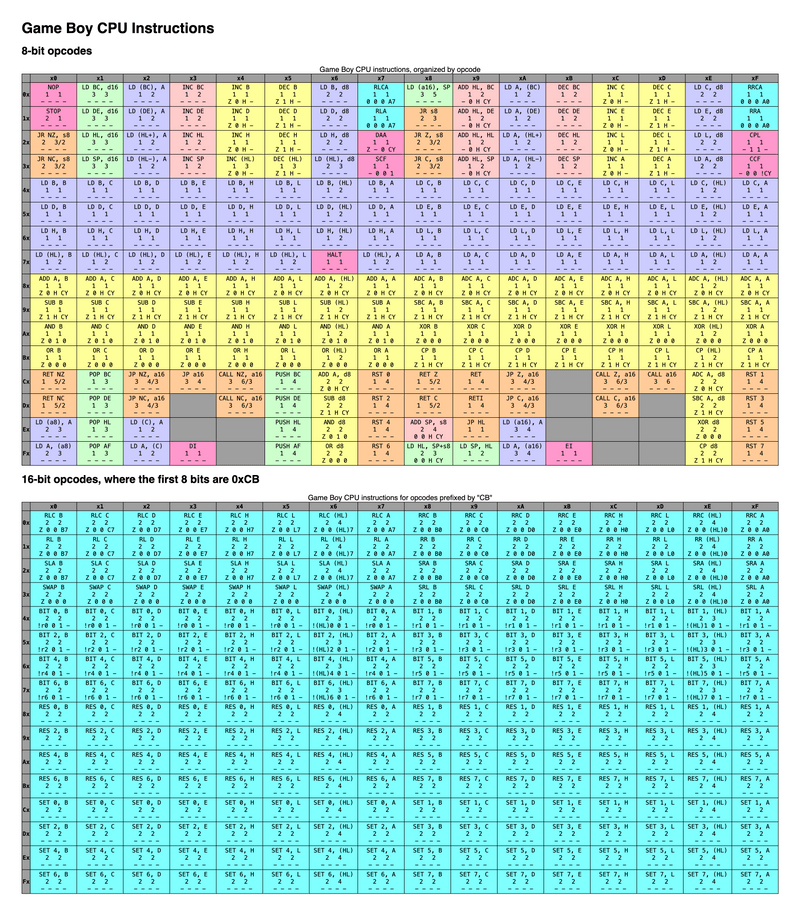
\includegraphics[width=1\textwidth]{./images/opcodes.png}
\centering
\caption{Gameboy's opcode-tables}
\label{fig:opcode-tables}

\end{figure}

\end{document}
